\documentclass[stochastic-or.tex]{subfiles}
\usepackage{amsmath} % this is only used to enforce good environment completion in emacs
\externaldocument{stochastic-or}

\loadgeometry{tufte}

\begin{document}

\section{Poisson Arrivals See Time Averages}
\label{sec:poisson-arrivals-see}

Suppose jobs arrive exactly at the start of an hour and require 59 minutes of service.
If we sample the server occupation at job arrival times, the server is always free as seen by the arrivals, while if we track the server over time, it is nearly always busy.
Thus, what jobs see upon arrival is \emph{in general not equal} to what the server perceives.
However, when jobs arrive as a Poisson process, both sampling methods produce the same number, a result known as the \recall{Poisson arrivals see time averages} (\recall{PASTA}) property.
Here we will discuss this property in more detail, and in the remainder of the book we will use it time and again.

\newthought{Let us say} that the system is in \emph{state}~$n$ at time~$t$ when $L(t)=n$. Then define\marginnote{Note the $A_k-$; since $L(t)$ is right-continuous, we concentrate on what an \emph{arrival} sees just before it's arrival}
\begin{equation}\label{eq:rates_}
 A(n,t) :=  \sum_{k=1}^\infty \1{A_k \leq t}\1{\L(A_k-) = n} = \sum_{k=1}^{A(t)}\1{\L(A_k-) = n}
\end{equation}
as the number of arrivals up to time~$t$ that saw the system in state~$n$.\marginnote{\cref{ex:36},\cref{ex:38}}
Next, let
\begin{equation*}
 Y(n,t) := \int_0^t \1{\L(s) = n} \d s
\end{equation*}
be the total time the system spends in state~$n$ during $[0,t]$.
% , and
% \begin{equation} \label{eq:18}
%  p(n,t) := \frac 1 t \int_0^t \1{\L(s) = n} \d s = \frac{Y(n,t)}t,
% \end{equation}
% \end{subequations}
% be the fraction of time in state~$n$ during $[0,t]$.
To see the practical relevance of this definitions, suppose it costs~$w$ per unit time to have a job in the system.
Then, the total cost up to time~$t$ is $w \sum_{n=0}^\infty n Y(n,t)$. % and the time-average cost is $w \sum_{n=0}^\infty n p(n,t)$.
\begin{marginfigure}%[t]
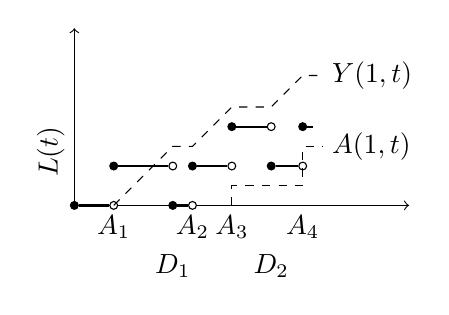
\begin{tikzpicture}[scale=0.5,
 open/.style={shape=circle, fill=white, inner sep=1pt, draw, node contents=},
 closed/.style={shape=circle, fill=black, inner sep=1pt, draw, node contents=},
]

%axis
\draw[->] (0,0) -- coordinate (x axis mid) (8.5,0);
\draw[->] (0,0) -- coordinate (y axis mid) (0,4.5);
%\node[below=0.2cm] at (x axis mid) {$t$};
\node[left=0.3cm, rotate=90] at (y axis mid) {$L(t)$};


\draw
node (0) at (0,0) [closed] {}
node (c1) at (1,0) [open] {};
\draw[thick] (0)--(c1);
\node[below] at (1,0) {$A_1$};

\draw
node (c2) at (1,1) [closed] {}
node (c3) at (2.5,1) [open] {};
\draw[thick] (c2)--(c3);
\node[below] at (2.5,-1) {$D_1$};

\draw
node (c2) at (2.5,0) [closed] {}
node (c3) at (3,0) [open] {};
\draw[thick] (c2)--(c3);
\node[below] at (3,0) {$A_2$};

\draw
node (c2) at (3,1) [closed] {}
node (c3) at (4,1) [open] {};
\draw[thick] (c2)--(c3);

\draw
node (c2) at (4,2) [closed] {}
node (c3) at (5,2) [open] {};
\draw[thick] (c2)--(c3);
\node[below] at (4,0) {$A_3$};

\draw
node (c2) at (5,1) [closed] {}
node (c3) at (5.8,1) [open] {};
\draw[thick] (c2)--(c3);
\node[below] at (5.,-1) {$D_2$};

\draw
node (c2) at (5.8,2) [closed] {}
node (c3) at (6.3,2) {};
\draw[thick] (c2)--(c3);
\node[below] at (5.8,0) {$A_4$};

\draw[dashed] (1,0)--(2.5, 1.5) -- (3, 1.5)--(4,2.5) --
(5, 2.5)--(5.8, 3.3)--(6.3, 3.3);
\node[right] at (6.3, 3.3) {$Y(1,t)$};

\draw[dashed] (4,0) -- (4,0.5)--(5.8, 0.5)--(5.8, 1.5)--(6.3, 1.5);
\node[right] at (6.3, 1.5) {$A(1,t)$};

\end{tikzpicture}
\footnotesize{\emph{We subtracted $1/2$ from the graph of $A(1,t)$, for otherwise this  overlaps with the graph of~$Y$.}}
\end{marginfigure}

With these definitions, assume the following limits exist:
\begin{subequations}
\label{eq:18}
\begin{align}
\lambda &:= \lim_{t\to\infty} \frac{A(t)}{t}, & \lambda(n) &:= \lim_{t\to\infty} \frac{A(n,t)}{Y(n,t)}, \\
p(n) &:=\lim_{t\to\infty} \frac{Y(n,t)}{t},  & \pi(n) &:= \lim_{t\to\infty}\frac1{A(t)}\sum_{k=1}^{A(t)} \1{\L(A_k-) = n}.
\end{align}
\end{subequations}
Here, $\lambda(n)$ has the interpretation of the arrival rate \emph{while} the system is in state~$n$, $p(n)$ is the long-run fraction of \emph{time} spent in state~$n$, and $\pi(n)$ is the long-run fraction of \emph{arrivals} that observe~$n$ customers in the system.

\begin{theorem}\label{thr:4}
If all  limits exist, then,
\begin{equation}\label{eq:13}
\lambda \pi(n) = \lambda(n) p(n).
\end{equation}
\end{theorem}
\begin{proof}
% Let us write  $A(n,t)/t$ in two ways:
% \begin{equation}\label{eq:10444}
% \frac{A(n,t)}{Y(n,t)}\frac{Y(n,t)}t  = \frac{A(n,t)}t =  \frac{A(t)}t \frac{A(n,t)}{A(t)}.
% \end{equation}
% Taking the limit $t\to \infty$, we obtain for the LHS that the rate of arrivals that see the system in state~$n$ is equal to
On the one hand,
\begin{equation*}\label{eq:lc-3}
\lim_{t\to\infty} \frac{A(n,t)}t = \lim_{t\to\infty} \frac{A(n,t)}{Y(n,t)}\frac{Y(n,t)}t = \lambda(n) p(n).
\end{equation*}
On the other,
\begin{equation*}
\lim_{t\to\infty} \frac{A(n,t)}t = \lim_{t\to\infty} \frac{A(n,t)}{A(t)}\frac{A(t)}t = \pi(n) \lambda.
\end{equation*}
% For the RHS in~\cref{eq:10444}, it is clear that $A(t)/t\to \lambda$, so we need to interpret $A(n,t)/A(t)$.
% First, observe
% \begin{equation*}
% \frac{A(n,t)}{A(t)}
% % = \frac1{A(t)}\sum_{k=1}^\infty \1{A_k \leq t, L(A_k-) = n}
% =   \frac1{A(t)}\sum_{k=1}^{A(t)} \1{\L(A_k-) = n}.
% \end{equation*}
% Then, since $A(t)\to \infty$ as $t\to\infty$, it follows from the renewal reward theorem\marginnote{\cref{ex:18}} that the following limit can be defined:
% \begin{equation}\label{eq:pasta2}
% \pi(n) := \lim_{t\to\infty}\frac1{A(t)}\sum_{k=1}^{A(t)} \1{\L(A_k-) = n}.
% \end{equation}
% Finally, as in~\cref{eq:10444} the LHS and RHS are equal, the limits are the same. Hence,
\end{proof}

This result has a simple consequence.
Write $\mathcal{S}$ for all the states the system can attain.\marginnote{When there is no upper bound on $L$, then $\mathcal{S} = \N$, but when the $L$ is bounded by some number~$K$, then $\mathcal{S} = \{0, 1, \ldots, K\}$.}
Clearly, any arrival must see the system in some state, hence $\sum_{n\in \mathcal{S}} \pi(n) = 1$.
Thus, summing over~$n$ in~\cref{eq:13}, the overall arrival rate $\lambda$ is such that
\begin{equation}
\label{eq:lc-1}
\lambda = \sum_{n\in \mathcal{S}} \lambda(n)p(n).
\end{equation}


With this theorem we can obtain second result of utmost importance.
\begin{theorem}
If the arrival rate does not depend on the state of the system, i.e., $\lambda(n)=\lambda$, the sample probabilities $\{\pi(n)\}$ are equal to the time-average probabilities $\{p(n)\}$, i.e.,
\begin{equation}\label{eq:pasta}
 \lambda(n) = \lambda \iff \pi(n) = p(n).
\end{equation}
\end{theorem}
\begin{proof}
From~\cref{eq:13}, $\pi(n) = \lambda(n) p(n)/\lambda$. By the assumption, $\lambda=\lambda(n)$, so the $\lambda$'s cancel.
\end{proof}


As the example in the introduction of this section shows, this property is not satisfied in general.
However,\marginnote{A rigorous proof of this is hard, see e.g., \cite{el-taha98:_sampl_path_analy_queuein_system}}
\begin{corollary}[Poisson Arrivals See Time Averages (PASTA)]
If the arrival process is Poisson, then $\lambda(n)=\lambda$, in which case $\pi(n)=p(n)$.
\end{corollary}



\newthought{By discretizing time} we can provide a simple and intuitive way to understand when PASTA does (not) hold.
%In a discrete-time queueing system, the event ${L(A_n-)=m}$ has the following interpretation.
If in some period~$n$ a job arrives, i.e., $a_{n}=1$, and the system contains~$m$ jobs at the end of the previous period, i.e., $L_{n-1}=m$, then we would say that the arrival sees $m$ jobs in the system upon arrival.
Thus, for $n$ large, $\pi(m) \approx \P{L_{n-1}=m | a_n=1}$.
Now, with Bayes' law:
\begin{equation*}
\P{L_{n-1}=m | a_n=1} = \frac{\P{a_n=1, L_{n-1}=m}}{\P{a_n=1}}.
\end{equation*}
Observing that $L_{n-1}$ is a function of $\{a_i\}_{i=1}^{n-1})$, then, when $a_{n}$ is independent of $\{a_i\}_{i=1}^{n-1}$, $a_{n}$ and $L_{n-1}$ are independent.
In that case $\P{a_n=1, L_{n-1}=m} = \P{a_n=1} \P{L_{n-1}=m}$, and by canceling $\P{a_{n}=1}$ in the fraction, we see that
\begin{equation*}
\pi(m) \approx \frac{\P{a_n=1} \P{L_{n-1}=m}}{\P{a_n=1}} = \P{L_{n-1}=m} \approx p(m),
\end{equation*}
where the last approximation follows from the fact that $\P{L_{n-1}=m}$ is the fraction of time $L_{n-1}=m$.\marginnote{For  mathematically interested students: The  assumed strong convergence $N^{-1}\sum_{n=1}^N \1{L_n=m} \to p(m)$ as $N\to\infty$ implies the weak converge $\P{L_n=m} \to p(m)$ as $n \to \infty$.}

However, PASTA does not hold when $a_{n}$ depends on $L_{n-1}$. For instance, if $a_{n}=0$ when $L_{n-1}>0$, and $c_{k}\sim \Bern{d}$ for some small probability~$d$, then $\pi(1) = 0$, but $\P{L_{n-1}=0} > 0$ in general.


\newthought{With just PASTA}, Little's law and memorylessness we can already achieve quite a few interesting results for the $M/M/1$ queue.\marginnote{For the $M/G/1$ queue, things are bit subtler, see \cref{ex:l-216} and~\cref{sec:n-policies-mg1}.}
First observe that
\begin{equation*}
 \E\J \stackrel 1 = \E \L \E S + \E S \stackrel 2= \lambda \E \J \E S + \E S \stackrel= \rho \E \J + \E S,
\end{equation*}
where $1$ follows from PASTA, 2 from Little's law $\E L = \lambda \E J$, and 3 from $\rho=\lambda\E S$.
Consequently,
\begin{subequations}
\begin{align}
 \E\J = \frac{\E S}{1-\rho},
\end{align}
and then step by step,
\begin{align}
 \E \L &= \lambda \E\J = \frac{\lambda \E S}{1-\rho} = \frac\rho{1-\rho}, \\
 \E{\W} &= \E L \E S = \frac{\rho}{1-\rho} \E S \label{eq:wqes}\\
 \E{\QQ} &= \lambda \E{\W} = \frac{\rho^2}{1-\rho}, \\
 \E{\Ls} &= \E \L - \E{\QQ} = \frac{\rho}{1-\rho} - \frac{\rho^2}{1-\rho} = \rho,
\end{align}
\end{subequations}


\newthought{To let you} think a bit deeper about the PASTA property, and statistics in general, consider the next interesting riddle.
The problem is known as the `inspection paradox'.\marginnote{ Look this paradox up on the web. You should be aware of such biases in data science.}[-0.7cm]

In a small Midwestern town\marginnote{The story comes  from the book `Puzzle Math' by G. Gamow and M. Stern, \url{https://www.arvindguptatoys.com/arvindgupta/puzzlemath.pdf}. The interesting solution can also be found there.}
 there lived a retired railroad engineer named William
Johnson.
The main line on which he had worked for so many years passed through the
town. Mr. Johnson suffered from insomnia and would often wake up at any odd hour of
the night and be unable to fall asleep again. He found it helpful, in such cases, to take a
walk along the deserted streets of the town, and his way always led him to the railroad
crossing. He would stand there thoughtfully watching the track until a train thundered by
through the dead of the night. The sight always cheered the old railroad man, and he
would walk back home with a good chance of falling asleep.

After a while he made a curious observation; it seemed to him that most of the trains he saw at the crossing were traveling eastward, and only a few were going west.
Knowing very well that this line was carrying equal numbers of eastbound and westbound trains, and that they alternated regularly, he decided at first that he must have been mistaken in this reckoning.
To make sure, he got his little notebook, and began putting down “E” or “W,” depending on which way the first train to pass was traveling.
At the end of a week, there were five “E’s” and only two “W’s” and the observations of the next week gave essentially the same proportion.
Could it be that he always woke up at the same hour of night, mostly before the passage of eastbound trains?

Being puzzled by this situation, he decided to undertake a rigorous statistical study of the problem, extending it also to the daytime.
He asked a friend to make a long list of arbitrary times such as 9:35 a.m., 12:00 noon, 3:07 p.m., and so on, and he went to the railroad crossing punctually at these times to see which train would come first.
However, the result was the same as before.
Out of one hundred trains he met, about seventy-five were going east and only twenty-five west.
In despair, he called the depot in the nearest big city to find whether some of the westbound trains had been rerouted through another line, but this was not the case.
He was, in fact, assured that the trains were running exactly on schedule, and that equal numbers of trains daily were going each way.
This mystery brought him to such despair that he became completely unable to sleep and was a very sick man.

Can you reveal the mystery thereby solving the sleeping problems of Mr. Johnson?


\begin{truefalse}
Claim:  the PASTA property implies  that $\sum_{n=0}^\infty n p(n) = \sum_{n=0}^\infty n \pi(n)$ for any $G/M/1$ queue.
\begin{solution}
False. In the $G/M/1$ queue jobs don't arrive as a Poisson process.
\end{solution}
\end{truefalse}

\begin{truefalse}
Consider a stable $M/G/1$ queue.
Claim: By the PASTA property, a fraction~$\rho$ of the arrivals sees the server occupied, while a fraction $1-\rho$ sees a free server.
\begin{solution}
True.
\end{solution}
\end{truefalse}

\begin{truefalse}
Claim: For the $M/G/1$ queue it follows from the PASTA property that
 \begin{equation*}
\E J = \sum_{n=0}^\infty \E{W \given L=n} \pi(n) + \E S.
 \end{equation*}
\begin{solution}
True.
\end{solution}
\end{truefalse}

\begin{truefalse}
Let $L_{S}(s)$ be the number of items in the system at time $s$.
Define
\begin{equation*}
\alpha = \lim_{n\to\infty} \frac 1 n \sum_{k=1}^n L_{S}(A_k).
\end{equation*}
For the $M/G/1$ queue we can use PASTA to see that $1-\rho = \alpha$.
\begin{solution} False, for various reasons. First we should use  $L(A_{k}-)$ instead of $L(A_{k})$ to count the number of arrivals seen \emph{upon arrival}.  Seccond, $\alpha$ counts the fraction of arrivals that see the number of jobs at the server (not in the system). By PASTA this must be the load, which is $\rho$; $1-\rho$ is the fraction of time the server is idle.

BTW, here is another way to write $\alpha$:
\begin{equation*}
\alpha = \lim_{n\to\infty} \frac 1 n \sum_{k=1}^n \1{L(A_k-) > 0} = \lim_{t\to\infty} \frac{1}{t}\int_0^{t} \1{L(s) > 0}\d s.
\end{equation*}
\end{solution}
\end{truefalse}

\begin{exercise}\label{ex:36}
Removed.
\end{exercise}

\begin{exercise} \label{ex:38}
If $\lambda>\delta$, can it happen that $ \lim_{t\to\infty} A(n,t)/t > 0$ for some (finite)~$n$?
\begin{solution}
If $\lambda > \delta$, then $L(t)\to\infty$.
But then there must be a last time, $s$ say, that $L(s) = n+1$, and $L(t) > n+1$ for all $t>s$.
Hence, after time~$s$ there will never be a job that will see the system with~$n$ jobs.
Thus $A(n,t) = A(n,s)$ for all $t>s$ (recall, $A(n,t)$ can only change at time $t$, say, when a job arriving at $t$ sees $n$ in the system.
But since $L(t) > n+1$ for $t>2$, this will never happen after $ts$.)
As $A(n,t)$ remains finite, $\lim_{t\to\infty}A(n,t)/t=0$.
\end{solution}
\end{exercise}


\begin{exercise}\label{ex:26}
 When $\lambda\neq \delta$, is $\pi(n)\geq \delta(n)$?
\begin{hint}
Solve \cref{ex:38} first.
Use that $\lambda \geq \delta$ always holds.
Thus, when $\lambda \neq \delta$, it must be that $\lambda > \delta$.
What are the consequences of this inequality; how does the queue length behave as a function of time?
\end{hint}
\begin{solution}
 The assumptions lead us to conclude that $\lambda > \delta$. As a consequence, the queue length must increase in the long run (jobs come in faster than they leave). Therefore, $A(n,t)/t \to 0$ for all~$n$, and also $D(n,t)/t\to 0$. Consequently, $\pi(n) = \delta(n) = 0$, which is the only sensible reconciliation with~\cref{eq:36}.
\end{solution}
\end{exercise}



% \begin{exercise}\label{ex:18}
% Suppose that the limit $A(n,t)/t \to Y$ exists as $t\to \infty$. Use this and  the renewal-reward theorem to explain that $A(n,t)/t \to \lambda \pi(n)$.
% \begin{hint}
% Check that the conditions of the renewal reward theorem are satisfied in the above proof of~\cref{eq:pasta2}. Then define
% \begin{align*}
%  Y(t) &:= A(n,t) = \sum_{k=1}^{A(t)} \1{\L(A_k-) = n} \\
% X_k &:= Y(A_k) - Y(A_{k-1}) = A(n, A_k) - A(n, A_{k-1}) = \1{\L(A_k-)=n}.
% \end{align*}

% \end{hint}
% \begin{solution}
% First we check the conditions. The counting process here is $\{A(t)\}$ and the epochs at which
%  $A(t)$ increases are $\{A_k\}$. By assumption, $A_k\to\infty$,
%  hence $A(t)\to\infty$ as $t\to\infty$. Moreover, by assumption
%  $A(t)/t \to \lambda$. Also, $A(n,t)$ is evidently non-decreasing and
%  $A(n,t)\to\infty$ as $t\to\infty$.


% From the definitions in the hint,
% \begin{equation*}
% X= \lim_{m\to\infty} \frac 1 m \sum_{k=1}^m X_k =\lim_{m\to\infty} \frac 1 m \sum_{k=1}^m \1{\L(A_k-)=n} = \pi(n).
% \end{equation*}
% Since $Y=\lim_{t\to\infty} Y(t)/t = \lim_{t\to\infty} A(n,t)/t$ it follows from the renewal reward theorem that
% \begin{equation*}
%  Y=\lambda X \implies \lim_{t\to\infty} \frac{A(n,t)} t = \lambda X = \lambda \pi(n).
% \end{equation*}
% \end{solution}
% \end{exercise}



\begin{exercise}\label{ex:l-216}
While~\cref{eq:wqes} is true for the $M/M/1$, it is \emph{not true for the $M/G/1$ queue}. Why is that?
\begin{solution}
 By the memoryless property of the (exponential) distributed service times of the $M/M/1$ queue, the duration of a job in service, if any, is $\Exp{\mu}$ also at an arrival moment.
 Therefore, at an arrival moment, all jobs in the system (whether in service or not) have the same expected duration.
 Hence, the expected time to spend in queue is the expected number of jobs in the system times the expected service time of each job, i.e., $\E{\W} = \E \L \E S$.
 Note that we use PASTA to see that the expected number of jobs in the system at an arrival is $\E{\L}$.
 For the $M/G/1$ queue, the job in service (if any) does not have the same distribution as a job in queue.
 Hence, for the $M/G/1$ queue, the \emph{expected time in queue is not} $\E \L \E S$.
\end{solution}
\end{exercise}


\end{document}

